\section{Course Pages}
\subsection{Overview}
The course pages are a crucial component of any learning management system.
It is the place where students and academics mainly interact with the LMS and acts as the centralised page in which other components are linked, for example the lectures, tutorials and quizzes. 
The course pages also includes the course dashboard, course content and course selection pages. 
The course dashboard page is the home page for a course, it displays important announcements to notify students of important information.
The course content is the page where slides, tutorial questions and notes are found and the course selection page is where users have an overview of all of the courses they are enrolled in and provides them a way to navigate the MetaLMS.
These pages offer other bonus functionality such as widgets which will be discussed in further sections.

\subsection{Pages}
The main 3 pages that the course pages will encompass are:
\begin{itemize}
    \item The course dashboard
    \item The course content page
    \item The course selection page
\end{itemize}

\subsubsection{Course Dashboard page}
\begin{figure}[h]
    \centering
    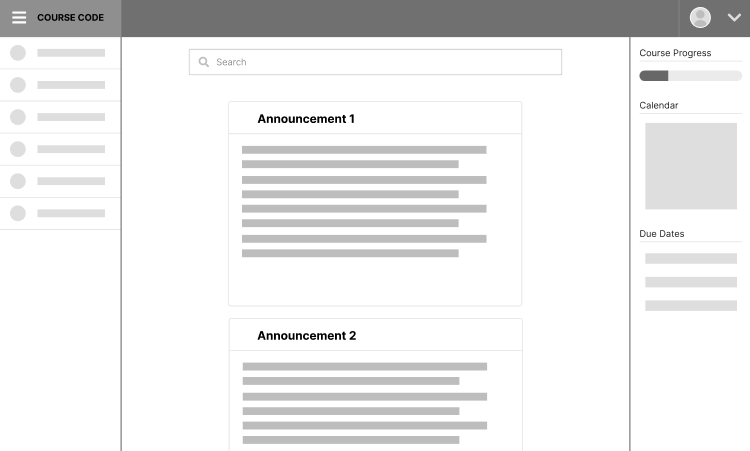
\includegraphics[scale=0.4]{course-pages-main}
    \caption{The main dashboard/page within the course.}
\end{figure}
\begin{figure}[h]
    \centering
    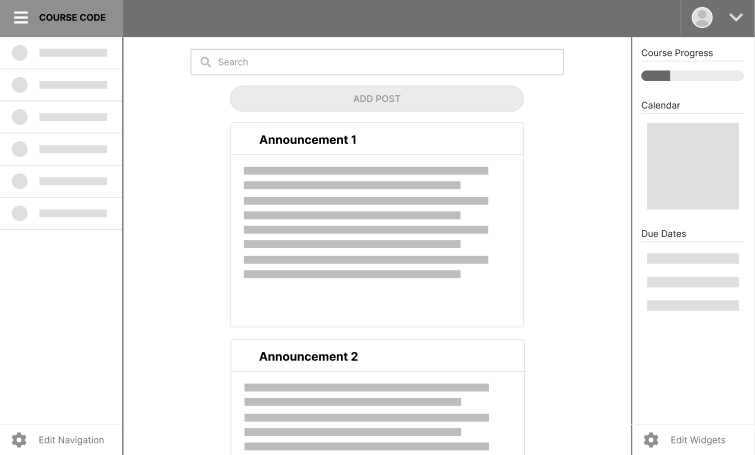
\includegraphics[scale=0.4]{course-pages-main-admin}
    \caption{The administrator view of the main dashboard/page.}
\end{figure}
The course dashboard is the centralised aspect of the course pages.
This page provides users with somewhat of a default home page for a particular course.
Within this page there will be a main dashboard/feed, a sidebar which links users to different aspects of the course and customisable widgets which provide further functionality. 

The main dashboard acts as the display of all announcements by administrator and academics. Administrators and academics are able to create announcements in which all users in the corresponding course can view. 
Announcements are crucial to a course as they provide an efficient method of communication between administrators, academics and students/users.
Users creating announcements will be able to attach files and links to better improve the usability of the planned LMS.
Within each announcement, users will also be able to create comments which are linked to the forums.

The sidebar for the dashboard page is a component within the page that provides the user with the ability to navigate through other aspects of the LMS.
Currently the components that will be linked in the sidebar are:
\begin{itemize}
    \item Course Content;
    \item Course Forum;
    \item Lectures;
    \item Tutorials.
\end{itemize}

The final component of the main page is the widgets bar. These widgets offer more extensive usability and utility for users of the LMS.
Some features that they offer are a course progress tracker and a calendar for users to view course due dates. 

\subsubsection{Course Content Page}
\begin{figure}[h]
    \centering
    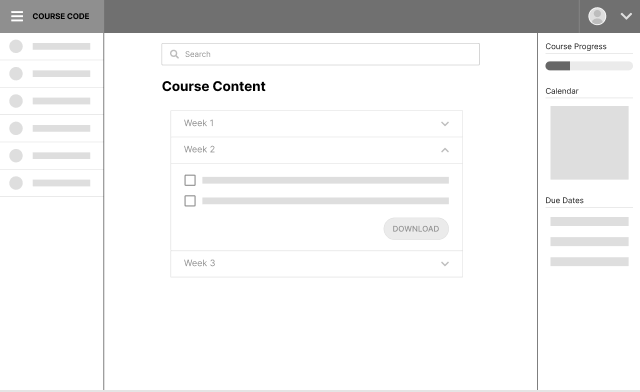
\includegraphics[scale=0.5]{course-pages-content}
    \caption{The course content page within the course.}
\end{figure}
\begin{figure}[h]
    \centering
    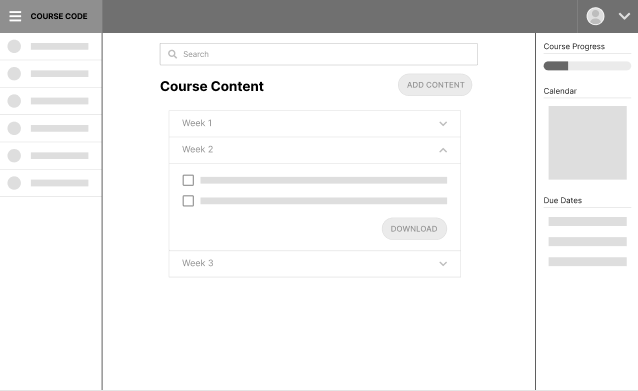
\includegraphics[scale=0.5]{course-pages-content-admin}
    \caption{The administrator view of the course content page.}
\end{figure}
The course content page is the area in which content is uploaded by administrators or academics and downloaded, viewed or completed by students.
The course content page will contain content from the topic tree and will be catergorised accordingly. 
One assumption made for the topic tree component is that the topic tree will be utilised as a database which stores content that can be utilised in courses.
Course administrators would have the ability to select which content to import into the course content page. 
The topic content will be categorised into 4 distinct types (preparation, content, practice, assessments).
Course content involves the topics that will be stored within the topic tree. This can range from lecture slides, tutorial questions, lecture recordings an even quizzes and assignments. 

\subsubsection{Course Selection page}
\begin{figure}[h]
    \centering
    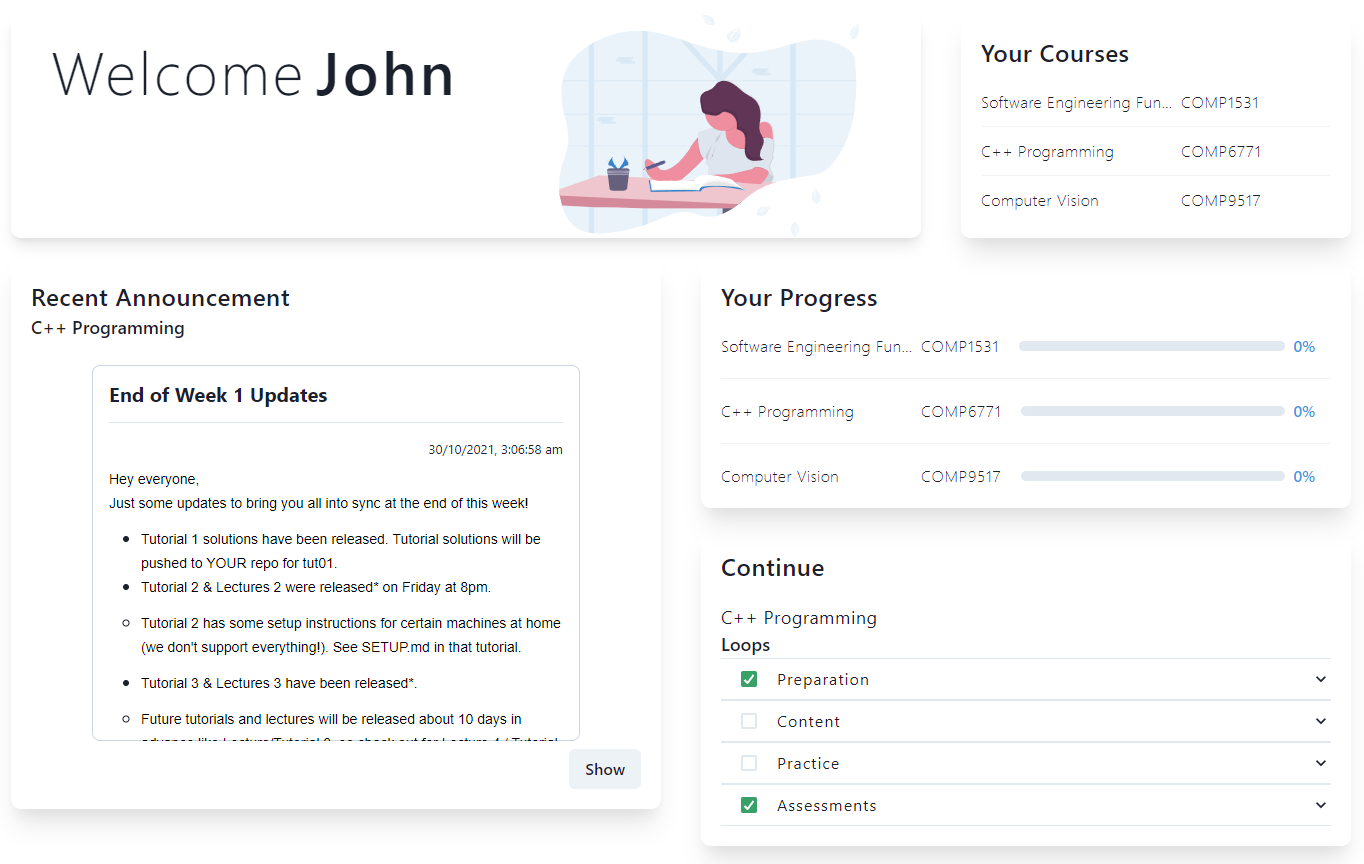
\includegraphics[scale=0.4]{course-selection-page}
    \caption{Student view of the course selection page}
\end{figure}
The course selection page is utilised as the central hub for users to have an overview of all of their enrolled courses.
It acts as the area of the MetaLMS to navigate to the topic tree, enrolments, courses and other features.
It also contains other features to provide utility for users to better their learning.

\subsection{Additional Features and Refinements}
The main changes that were implemented in Thesis B and Thesis C were the addition of the course selection page and the removal of the course outline page.
The course outline page was deemed low priority as it would not encompass high priority use cases and the course selection page was more deemed more crucial.
The previous plan was to develop only the course outline page, course content page and the course dashboard page.
Without the course selection page, a user would not have the ability to transition to different courses.
However with further development, the course outline page can be implemented.

\subsection{Requirements}
The requirements and use cases for the course pages are outlined below.
These features are prioritiesed using the MoSCoW method which assists with identifying the order to implement requirements.

\subsubsection{Functional Requirements}

\textbf{Course Selection Page}
\FloatBarrier
\begin{table}[h!]
    \begin{tabular}{|l|l|}
        \hline
        \textit{As a} & User \\ \hline
        \textit{I want to} & View my enrolled courses \\ \hline
        \textit{So that} & I can see what classes I am enrolled in \\ \hline
        \textit{Priority} & {\color[HTML]{FE0000} High} \\ \hline
        \textit{Status} & Complete \\ \hline
    \end{tabular}
\end{table}

\begin{table}[h!]
    \begin{tabular}{|l|l|}
        \hline
        \textit{As a} & User \\ \hline
        \textit{I want to} & Select a course I wish to navigate to \\ \hline
        \textit{So that} & I can navigate to the course pages of the corresponding course and begin studying \\ \hline
        \textit{Priority} & {\color[HTML]{FE0000} High} \\ \hline
        \textit{Status} & Complete \\ \hline
    \end{tabular}
\end{table}

\begin{table}[h!]
    \begin{tabular}{|l|l|}
        \hline
        \textit{As a} & User \\ \hline
        \textit{I want to} & View my progress for an enrolled course \\ \hline
        \textit{So that} & I can determine any courses that I may need to complete\\ \hline
        \textit{Priority} & {\color[HTML]{3166FF} Low} \\ \hline
        \textit{Status} & Complete \\ \hline
    \end{tabular}
\end{table}

\begin{table}[h!]
    \begin{tabular}{|l|l|}
        \hline
        \textit{As a} & User \\ \hline
        \textit{I want to} & View the most recent announcements from my enrolled courses \\ \hline
        \textit{So that} & I quickly see the most recent notification and be alert to any changes \\ \hline
        \textit{Priority} & {\color[HTML]{FE996B} Medium} \\ \hline
        \textit{Status} & Complete \\ \hline
    \end{tabular}
\end{table}

\begin{table}[h!]
    \begin{tabular}{|l|l|}
        \hline
        \textit{As a} & User \\ \hline
        \textit{I want to} & Be able to access my most recently accessed topic \\ \hline
        \textit{So that} & I can quickly continue my studies without needing to navigate to the course page \\ \hline
        \textit{Priority} & {\color[HTML]{3166FF} Low} \\ \hline
        \textit{Status} & Complete \\ \hline
    \end{tabular}
\end{table}

\begin{table}[h!]
    \begin{tabular}{|l|l|}
        \hline
        \textit{As an} & Administrator \\ \hline
        \textit{I want to} & Be able to access the forums and enrollements of a course \\ \hline
        \textit{So that} & I can quickly access these features without needing extra navigation \\ \hline
        \textit{Priority} & {\color[HTML]{3166FF} Low} \\ \hline
        \textit{Status} & Complete \\ \hline
    \end{tabular}
\end{table}

\pagebreak
\FloatBarrier
\textbf{Course Dashboard Page}
\FloatBarrier
\begin{table}[h!]
    \begin{tabular}{|l|l|}
        \hline
        \textit{As a} & User \\ \hline
        \textit{I want to} & View the announcements of a course \\ \hline
        \textit{So that} & I can see any important notifications for a particular course \\ \hline
        \textit{Priority} & {\color[HTML]{FE0000} High} \\ \hline
        \textit{Status} & Complete \\ \hline
    \end{tabular}
\end{table}

\begin{table}[h!]
    \begin{tabular}{|l|l|}
        \hline
        \textit{As an} & Administrator \\ \hline
        \textit{I want to} & Be able to create announcements \\ \hline
        \textit{So that} & I can notify enrolled students of important information \\ \hline
        \textit{Priority} & {\color[HTML]{FE0000} High} \\ \hline
        \textit{Status} & Complete \\ \hline
    \end{tabular}
\end{table}

\begin{table}[h!]
    \begin{tabular}{|l|l|}
        \hline
        \textit{As an} & Administrator \\ \hline
        \textit{I want to} & Be able to edit announcements \\ \hline
        \textit{So that} & I can change an announcement if any information is out of date or has changed \\ \hline
        \textit{Priority} & {\color[HTML]{FE996B} Medium} \\ \hline
        \textit{Status} & Complete \\ \hline
    \end{tabular}
\end{table}

\begin{table}[h!]
    \begin{tabular}{|l|l|}
        \hline
        \textit{As a} & User \\ \hline
        \textit{I want to} & Be able comment on an announcement \\ \hline
        \textit{So that} & I can ask for clarification or ask a question about the announcement \\ \hline
        \textit{Priority} & {\color[HTML]{FE996B} Medium} \\ \hline
        \textit{Status} & Complete \\ \hline
    \end{tabular}
\end{table}

\begin{table}[h!]
    \begin{tabular}{|l|l|}
        \hline
        \textit{As a} & User \\ \hline
        \textit{I want to} & Be able filter announcements \\ \hline
        \textit{So that} & I can search for a specific announcement for information\\ \hline
        \textit{Priority} & {\color[HTML]{FE996B} Medium} \\ \hline
        \textit{Status} & Complete \\ \hline
    \end{tabular}
\end{table}

\pagebreak
\FloatBarrier
\textbf{Course Content Page}
\FloatBarrier
\begin{table}[h!]
    \begin{tabular}{|l|l|}
        \hline
        \textit{As a} & User \\ \hline
        \textit{I want to} & Be able to view topics and their corresponding topic files \\ \hline
        \textit{So that} & I can view what content this topic group contains\\ \hline
        \textit{Priority} & {\color[HTML]{FE0000} High} \\ \hline
        \textit{Status} & Complete \\ \hline
    \end{tabular}
\end{table}

\begin{table}[h!]
    \begin{tabular}{|l|l|}
        \hline
        \textit{As a} & User \\ \hline
        \textit{I want to} & Be able to view and download topic files \\ \hline
        \textit{So that} & I can save the content and complete it in my own time\\ \hline
        \textit{Priority} & {\color[HTML]{FE0000} High} \\ \hline
        \textit{Status} & Complete \\ \hline
    \end{tabular}
\end{table}

\begin{table}[h!]
    \begin{tabular}{|l|l|}
        \hline
        \textit{As a} & User \\ \hline
        \textit{I want to} & Be able convey I have completed a topic file \\ \hline
        \textit{So that} & I can determine what content I have not completed\\ \hline
        \textit{Priority} & {\color[HTML]{FE996B} Medium} \\ \hline
        \textit{Status} & Complete \\ \hline
    \end{tabular}
\end{table}

\begin{table}[h!]
    \begin{tabular}{|l|l|}
        \hline
        \textit{As a} & User \\ \hline
        \textit{I want to} & Be able to view the prerequisites of a topic \\ \hline
        \textit{So that} & I can determine what content I will need to complete first before continuing\\ \hline
        \textit{Priority} & {\color[HTML]{FE996B} Medium} \\ \hline
        \textit{Status} & Complete \\ \hline
    \end{tabular}
\end{table}

\begin{table}[h!]
    \begin{tabular}{|l|l|}
        \hline
        \textit{As a} & User \\ \hline
        \textit{I want to} & Be able to filter topics \\ \hline
        \textit{So that} & I can search for a particular topic I may want to complete\\ \hline
        \textit{Priority} & {\color[HTML]{FE996B} Medium} \\ \hline
        \textit{Status} & Complete \\ \hline
    \end{tabular}
\end{table}

\begin{table}[h!]
    \begin{tabular}{|l|l|}
        \hline
        \textit{As a} & User \\ \hline
        \textit{I want to} & Be able to filter topics \\ \hline
        \textit{So that} & I can search for a particular topic I may want to complete\\ \hline
        \textit{Priority} & {\color[HTML]{FE996B} Medium} \\ \hline
        \textit{Status} & Complete \\ \hline
    \end{tabular}
\end{table}

\begin{table}[h!]
    \begin{tabular}{|l|l|}
        \hline
        \textit{As an} & Administrator \\ \hline
        \textit{I want to} & Be able to add topics or topic files to the content page \\ \hline
        \textit{So that} & I can easily modify the content of the course \\ \hline
        \textit{Priority} & {\color[HTML]{FE996B} Medium} \\ \hline
        \textit{Status} & Not Complete \\ \hline
    \end{tabular}
\end{table}

\pagebreak
\FloatBarrier
\textbf{Sidebar}
\FloatBarrier
\begin{table}[h!]
    \begin{tabular}{|l|l|}
        \hline
        \textit{As a} & User \\ \hline
        \textit{I want to} & Be able to click on a link and navigate to the corresponding component \\ \hline
        \textit{So that} & I can navigate within the MetaLMS\\ \hline
        \textit{Priority} & {\color[HTML]{FE0000} High} \\ \hline
        \textit{Status} & Complete \\ \hline
    \end{tabular}
\end{table}

\begin{table}[h!]
    \begin{tabular}{|l|l|}
        \hline
        \textit{As an} & Administrator \\ \hline
        \textit{I want to} & Be able to customise the links on the sidebar \\ \hline
        \textit{So that} & I can create or delete certain components within the MetaLMS for a course\\ \hline
        \textit{Priority} & {\color[HTML]{3166FF} Low} \\ \hline
        \textit{Status} & Not Complete \\ \hline
    \end{tabular}
\end{table}

\FloatBarrier
\textbf{Widgets bar}
\FloatBarrier
\begin{table}[h!]
    \begin{tabular}{|l|l|}
        \hline
        \textit{As a} & User \\ \hline
        \textit{I want to} & Be able to view reminders on a calendar \\ \hline
        \textit{So that} & I can easily determine the number of days before an important date \\ \hline
        \textit{Priority} & {\color[HTML]{FE996B} Medium} \\ \hline
        \textit{Status} & Complete \\ \hline
    \end{tabular}
\end{table}

\begin{table}[h!]
    \begin{tabular}{|l|l|}
        \hline
        \textit{As a} & User \\ \hline
        \textit{I want to} & Be able to create reminders on the calendar \\ \hline
        \textit{So that} & I can not down important dates so that I will not forget \\ \hline
        \textit{Priority} & {\color[HTML]{FE996B} Medium} \\ \hline
        \textit{Status} & Complete \\ \hline
    \end{tabular}
\end{table}

\begin{table}[h!]
    \begin{tabular}{|l|l|}
        \hline
        \textit{As a} & User \\ \hline
        \textit{I want to} & Be able to delete reminders on the calendar \\ \hline
        \textit{So that} & I can remove unnecessary reminders \\ \hline
        \textit{Priority} & {\color[HTML]{FE996B} Medium} \\ \hline
        \textit{Status} & Complete \\ \hline
    \end{tabular}
\end{table}

\begin{table}[h!]
    \begin{tabular}{|l|l|}
        \hline
        \textit{As a} & User \\ \hline
        \textit{I want to} & Be able to edit reminders on the calendar \\ \hline
        \textit{So that} & I can update the information of a reminder in case the important event has changed \\ \hline
        \textit{Priority} & {\color[HTML]{3166FF} Low} \\ \hline
        \textit{Status} & Not Complete \\ \hline
    \end{tabular}
\end{table}

\begin{table}[h!]
    \begin{tabular}{|l|l|}
        \hline
        \textit{As a} & User \\ \hline
        \textit{I want to} & Be able to view the progress of a particular course \\ \hline
        \textit{So that} & I can easily see the amount of content I still need to complete \\ \hline
        \textit{Priority} & {\color[HTML]{FE996B} Medium} \\ \hline
        \textit{Status} & Not Complete \\ \hline
    \end{tabular}
\end{table}

\begin{table}[h!]
    \begin{tabular}{|l|l|}
        \hline
        \textit{As a} & User \\ \hline
        \textit{I want to} & Be able to customise what widgets are present on the widgets bar \\ \hline
        \textit{So that} & I can determine what widgets are on my widgets bar \\ \hline
        \textit{Priority} & {\color[HTML]{FE996B} Low} \\ \hline
        \textit{Status} & Not Complete \\ \hline
    \end{tabular}
\end{table}

\pagebreak
\FloatBarrier
\textbf{Course Outline Page}
\FloatBarrier
\begin{table}[h!]
    \begin{tabular}{|l|l|}
        \hline
        \textit{As a} & User \\ \hline
        \textit{I want to} & Be able to view the course outline of a particular course \\ \hline
        \textit{So that} & I can determine the learning outcomes of a course \\ \hline
        \textit{Priority} & {\color[HTML]{FE996B} Medium} \\ \hline
        \textit{Status} & Not Complete \\ \hline
    \end{tabular}
\end{table}

\begin{table}[h!]
    \begin{tabular}{|l|l|}
        \hline
        \textit{As an} & Administrator \\ \hline
        \textit{I want to} & Be able to upload a course outline to a particular course \\ \hline
        \textit{So that} & I can provide learning outcomes for a course \\ \hline
        \textit{Priority} & {\color[HTML]{FE996B} Medium} \\ \hline
        \textit{Status} & Not Complete \\ \hline
    \end{tabular}
\end{table}

\subsection{Evaluation}
The evaluation of the course pages will depend on a set criteria.
This criteria is proposed as followed:
\begin{itemize}
    \item Performance - Whether the course pages are fast and responsive;
    \item Accessibility - Can a wide array of users use the course pages easily;
    \item UI/UX - Is the feature easy to use and attractive; and,
    \item Errors - Is the feature bug and error free.
\end{itemize}

